\documentclass[a4paper,11pt]{report}
\usepackage[italian]{babel}
\usepackage[utf8]{inputenc}
\usepackage[total={170mm,267mm},top=15mm,bottom=15mm,left=21mm,right=21mm]{geometry}
\usepackage{graphicx}

\begin{document}

\begin{titlepage}
  \clearpage\thispagestyle{empty}
  \centering
  \vspace{1cm}
  {\normalsize Informatica - Area scientifica \\  Dipartimento di Scienze matematiche, informatiche e multimediali\\  Università di Udine \par}
  \vspace{3cm}
  {\Huge \textbf{Progetto di Social Computing}}\\
  \vspace{4cm}
  {\Large  Parata Loris (144338) \\ Arzon Francesco (142439)\\ Dal Fabbro Lorenzo (142300)\\ Galvan Matteo (142985) \\ }
  \vspace{12cm}
  {\normalsize Anno accademico 2020/2021}
  \pagebreak
\end{titlepage}

\tableofcontents{}
\pagebreak
\chapter{Sottografo di Twitter}
\section{Introduzione}
Questo primo progetto di Social Computing consiste nello studio della rete sociale di 5 utenti di Twitter.\\
Lo studio è stato svolto mediante la costruzione di un sottografo di Twitter, costituto da cinque nodi che rappresentano gli utenti principali e della loro relativa rete di contatti costituita dai loro follower, following e da rispettivi sottoinsiemi campionati in maniera random.
Nello specifico abbiamo analizzato la relazione diretta di \textbf{follows} tra tutti i nodi del grafo ed i cinque profili scelti.

\section{Costruzione del grafo}

\subsection{Download dei nodi}
Il primo passo consiste nello scaricare tutti i followers attraverso la \textbf{api.followers()} di Twitter dei cinque nodi principali:

\begin{itemize}
	\item @Mizzaro, @damiano10, @Miccighel\_, @eglu81, @KevinRoitero
\end{itemize}

\begin{figure}[h]
	\centering
	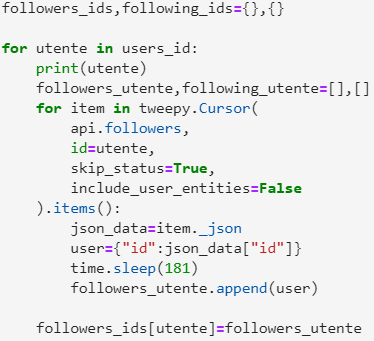
\includegraphics[width=0.4\linewidth]{followers}
	\label{fig:followers}
\end{figure}



\setlength{\parindent}{0pt}
L'uso della funzione \textbf{Cursor()} ci permette di restituire i dati richiesti ad una certa API in pagine. I parametri di questa funzione sono: \\
-\textbf{api.followers}: l'api desiderata, seguita dai parametri necessari ad essa.\\
-\textbf{id}: utente, indica l'id dello user "target" a cui siamo interessati\\
-\textbf{skip\_status= True}: in modo che gli stati non verranno inclusi negli oggetti utente restituiti.\\
-\textbf{include\_user\_entities= False}: in modo da non includere l'oggetto utente "entities"\\
\textbf{.items()} ci permette di indicare l'eventuale la grandezza desiderata del blocco di dati richiesto.\\ \medskip
Lo stesso procedimento è stato effettuato per i rispettivi following di ogni nodo principale, utilizzando la \textbf{api.friends()}.


\begin{figure}[h]
	\centering
	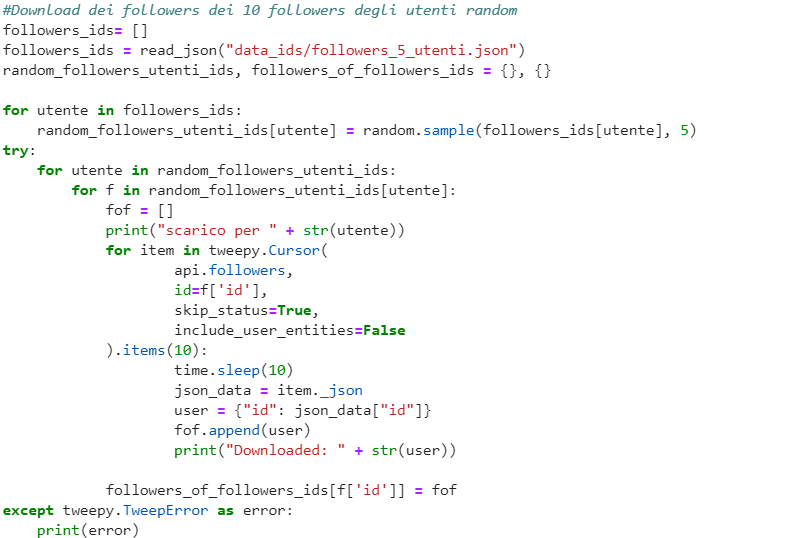
\includegraphics[width=0.8\linewidth]{random_followers}
	\label{fig:followers}
\end{figure}

Successivamente abbiamo selezionato gli \textbf{id} di 5 followers e 5 following randomicamente per ognuno dei 5 account. Da ognuno di essi sono stati scelti e scaricati gli id di altri 10 account followers e 10 account following sempre in maniera casuale.\\

Infine, una volta ottenuti tutti gli account, abbiamo scaricato tutte le informazioni principali relative agli account mediante la \textbf{api.get user()}, che ha come parametro l'\textbf{id} di un account precedentemente individuato.\\
\begin{figure}[ht]
	\centering
	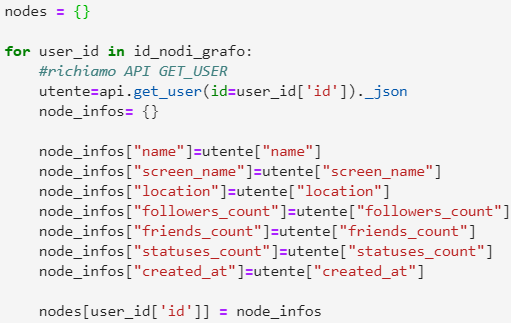
\includegraphics[width=0.4\linewidth]{api_get_user}
	\label{fig:apigetuser}
\end{figure}

Per un totale di \textbf{3103 nodi}.
\subsection{Creazione degli archi}
\begin{figure}[h]
	\centering
	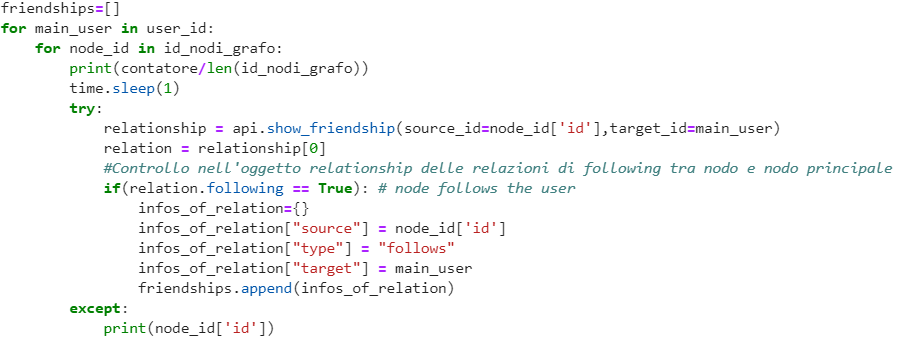
\includegraphics[width=0.8\linewidth]{api_show_friendships}
	\label{fig:apishowfriendships}
\end{figure}

Successivamente abbiamo controllato l'esistenza di una relazione tra tutti gli account scaricati ed i 5 nodi principali con la funzione \textbf{api.show\_friendship()}. Aggiungendo gli archi raffiguranti l'azione di follows un file json, indicando nodo sorgente, tipo di relazione e nodo target. Il try-catch è stato utilizzato per rilevare eventuali nodi problematici.\\
Questa operazione, essendo molto costosa temporalmente, è stata effettuata modificando il codice in maniera tale da poterlo eseguire, con chiavi di autenticazione developer diverse, per ogni singolo utente. In modo da parallelizzare l'operazione, che costava circa 5 ore di tempo per singolo utente, a causa dei limiti temporali di 180 richieste ogni 15 minuti di all'api Twitter. Tutti gli archi sono stati uniti in un unico file json. Abbiamo ottenuto un totale di \textbf{1922 archi}.
\subsubsection{Ottimizzazione archi}
E' possibile rilevare tutti i nodi direttamente connessi ai 5 account andando a visualizzare direttamente i rispettivi followers, con la \textbf{api.followers()}, riducendo significativamente i costi in termine di richieste all'API. Ma per attinenza alla traccia abbiamo fatto un controllo completo per ogni nodo scaricato precedentemente.
\subsection{Creazione del grafo}
La costruzione del grafo è stata effettuata mediante l'utilizzo delle funzioni messe a disposizione di networkx. 
\begin{figure}[h]
	\centering
	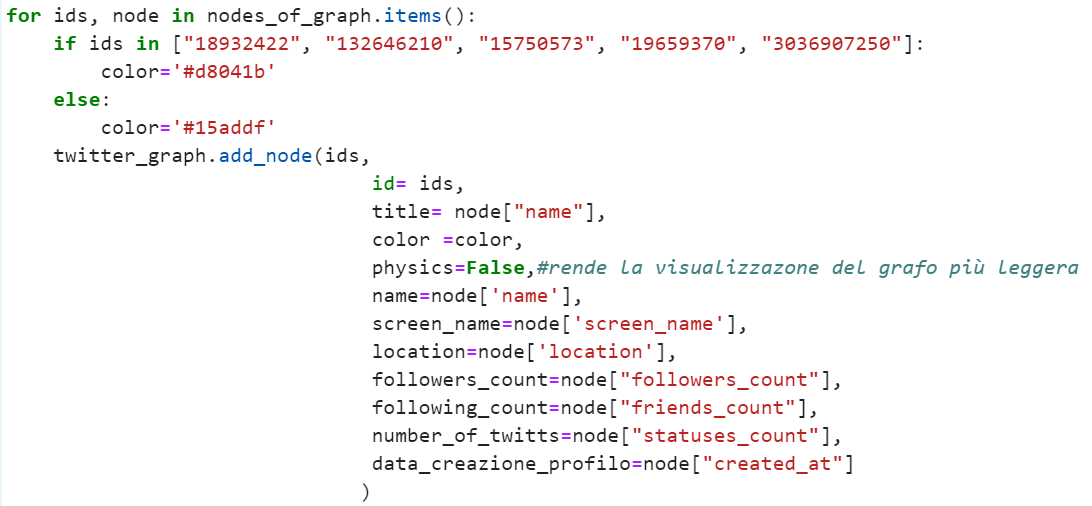
\includegraphics[width=0.7\linewidth]{aggiunta_nodi}
	\label{fig:aggiuntanodi}
\end{figure}
\\
Abbiamo inserito i nodi al grafo mediante la funzione \textbf{add\_node()}. Indicando come parametri:\\
-ids: identificatore del nodo\\
-id di visualizzazione\\
-title: il titolo visualizzato dal nodo\\
-colore: colore del nodo\\
-phisics: per abilitare o meno l'influenza del nodo sulla fisica del grafo\\
-i restanti attributi del nodo.
\newline

\begin{figure}[h]
	\centering
	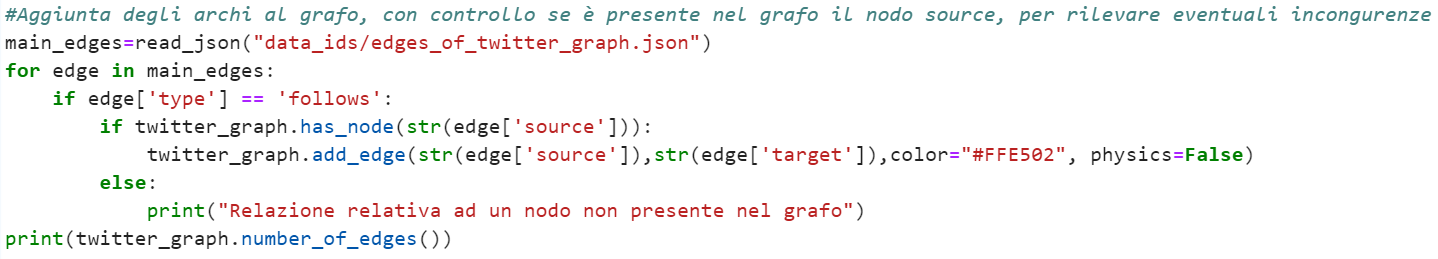
\includegraphics[width=0.8\linewidth]{aggiunta_archi}
	\label{fig:aggiuntaarchi}
\end{figure}

Mentre per aggiungere gli archi al grafo abbiamo controllato se è presente il nodo sorgente nel grafo con la funzione \textbf{has\_node()}, indicando l'id del nodo interessato, per rilevare eventuali incongurenze tra nodi scaricati e relazioni rilevate. Successivamente abbiamo aggiunto l'arco al grafo utilizzando la funzione \textbf{add\_edge()} indicando:\\
- nodo sorgente\\
- nodo target \\
- colore desiderato per l'arco durante la visualizzazione\\

\subsection{Visualizzazione del grafo}
La visualizzazione interattiva del grafo costruito con le funzioni messe a disposizione di networkX avviene utilizzando la libreria apposita pyvis. 
\subsubsection{Ottimizzazione visualizzazione}
E' possibile ridurre i costi per l'elaborazione grafica di costruzione del grafo impostando il parametro opzionale phisic = False. Questo parametro a discapito dell'interazione fisica nel trascinamento  dei nodi che avrebbero una risposta fisica, permette di risparmiare l'80 percento del tempo di rendering.

\section{Analisi del grafo completo}
Applicando le relative funzioni messe a disposizione dalla libreria di networkX abbiamo potuto stabilire che il grafo è:\\
Il grafo da noi analizzato è risultato \textbf{non connesso}.\\
Questo sottolinea che è errato dar per scontato che tutti gli utenti che seguono un determinato \\account \textbf{UtenteTwitter} a loro volta sono seguiti da utenti che seguono anche loro l' \textbf{UtenteTwitter}. \newline \\Nel caso in cui tenessimo traccia delle relazioni interne tra i nodi di secondo livello e quelli di terzo livello, considerando i path indiretti, allora sarebbe risultato connesso.\\ Ma questo dipende dalla componente casuale che sceglie da quali nodi scaricare i relativi follower dei follower.\newline
Ecco perchè abbiamo deciso di procedere alla rimozione dei nodi sconnessi del grafo principale e di confrontare le proprietà dei due grafi dove è possibile.

\subsection{Rimozione dei nodi sconnessi}
\begin{figure}[h]
	\centering
	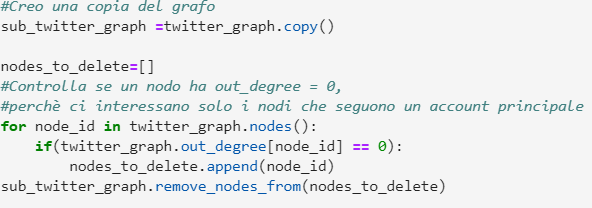
\includegraphics[width=0.6\linewidth]{rimozione_nodi_sconnessi}
	\label{fig:rimozionenodisconnessi}
\end{figure}
Questo codice ci permette di rimuovere dal grafo tutti i nodi che hanno \textbf{out-degree = 0}, cioè i nodi che non hanno archi uscenti.E nel nostro caso di ricerca dei follower,questa condizione basta per escludere i nodi sconnessi.\\
Otteniamo un grafo con soli \textbf{1679 nodi}.

\subsection{Proprietà dei grafi}
Il grafo completo risulta \textbf{non connesso}, mentre il suo sottografo è \textbf{connesso}.\\
Ma entrambi risultano \textbf{non bipartiti}.\\
Centro, Diametro e Raggio sono calcolabili solamente per il sottografo perchè il grafo completo essendo sconnesso ha valore di diametro e raggio infinito per definizione.\\
Per il sottografo abbiamo :
		\begin{itemize}
			\item Centro: ritroviamo i nodi di \textbf{Kevin Roitero}, \textbf{Gianluca Demartino} e \textbf{Damiano Spina},\\ tre dei 5 nodi principali.
			\item Diametro:  \textbf{4}
			\item Raggio: \textbf{2}
		\end{itemize}
\subsection{Misure di centralità}

Per le misure di Betweenness, Closness, Degree e In-centrality, otteniamo  valori massimi riferiti al nodo di damiano10, seguito da eglu81,Miccighel e dai restanti nodi principali.\\Per quanto riguarda l'out-centrality abbiamo come valore massimo un nodo che segue tre profili principali, per poi andare a decrescere per chi ne segue due e così via.
		\begin{itemize}
			\item Betweenness:\\ valore massimo: 0.000375 \\sottografo: 0.0012 
			\item Closness: \\valore massimo: 0.353 
			\\sottografo: 0.653
			\item Degree: \\valore massimo: 0.254 
			\\sottografo: 0.471
		\end{itemize}
		\begin{figure}[h]
		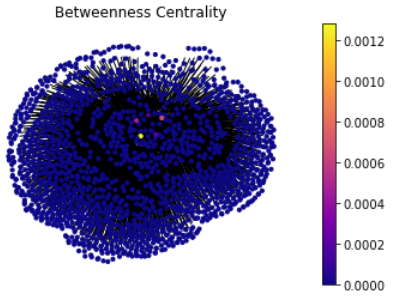
\includegraphics[width=.32\textwidth]{btw}\hfill
		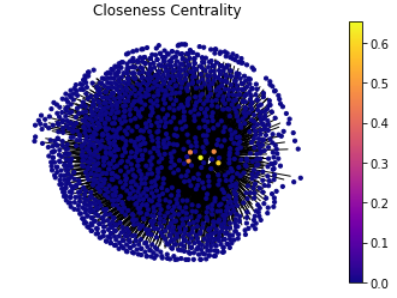
\includegraphics[width=.32\textwidth]{cls}\hfill
		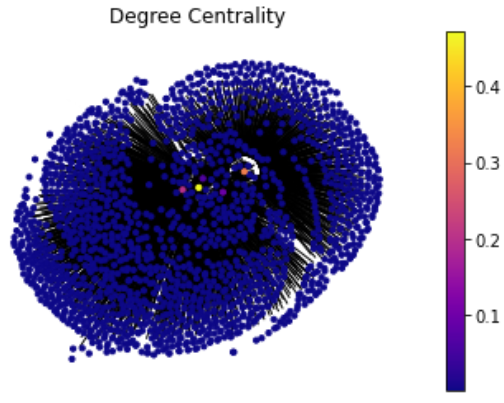
\includegraphics[width=.32\textwidth]{degree}
		\end{figure}
		\begin{itemize}
			\item In-centrality: 0.253 \\sottografo: 0.469
			\item Out-centrality: 0.00128 di Kevin Callegher \\sottografo: 0.00238 
		\end{itemize}
	\begin{figure}[h]
		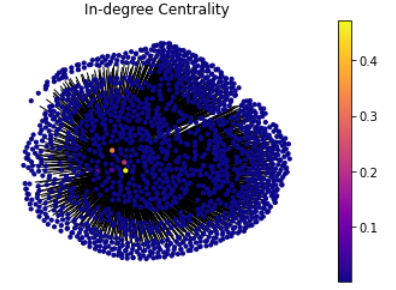
\includegraphics[width=.49\textwidth]{in-degree}\hfill
		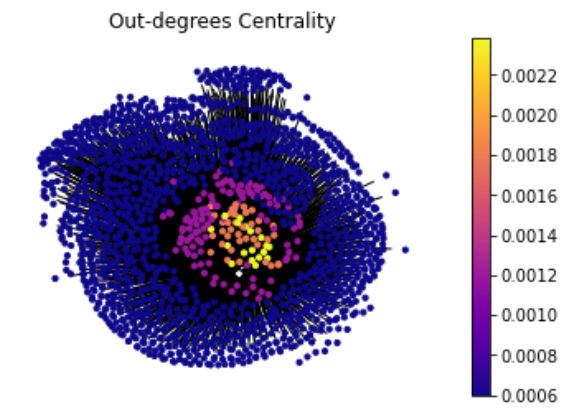
\includegraphics[width=.49\textwidth]{out-degree}
	\end{figure}

	Riportiamo anche i valori relativi al sottografo connesso perchè hanno un andamento coerente con il grafo grafo principale, ma i valori sono più alti perché abbiamo un numero di nodi complessivo minore.
		\begin{itemize}
			\item PageRank:\\ grafo completo: 0,216\\  
			sottografo: 0,243 \\per entrambi i valori si presentano in ordine al numero di followers che ogni account possiede.
			\item Hits: 
				\begin{itemize}
					\item Hubs: l'hub principale è Luke Gallagher, con valore 0.0015, che segue 3 profili su 5.
					\item Authorities: la maggiore autority è Damiano con valore di 0.624, seguito dai restanti nodi principali.
			\end{itemize}
		\end{itemize}
		\begin{figure}[h]
		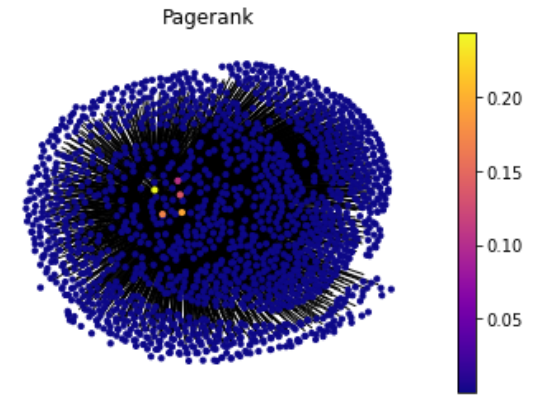
\includegraphics[width=.32\textwidth]{pagerank}\hfill
		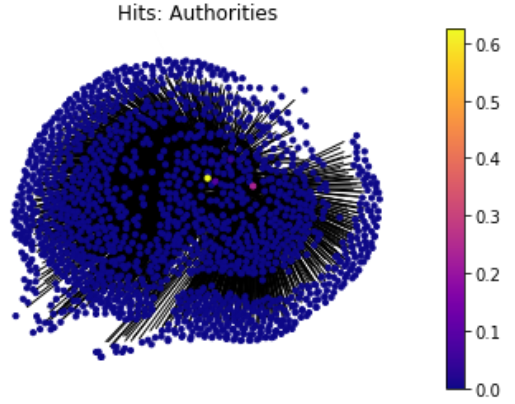
\includegraphics[width=.32\textwidth]{authorities}\hfill
		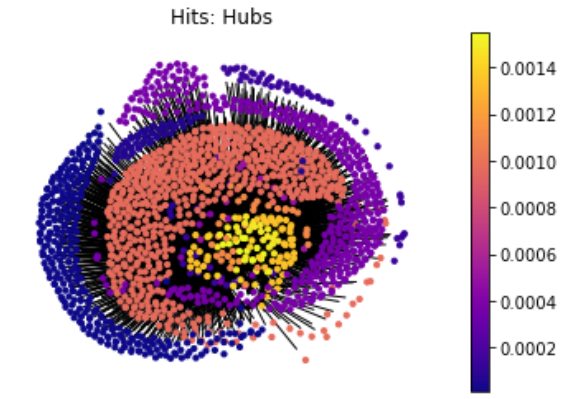
\includegraphics[width=.32\textwidth]{hubs}
		\end{figure}
	Dai risultati notiamo come l'algoritmo di \textbf{PageRank} sia influenzato dal numero di nodi complessivi rispetto a \textbf{HITS}. Inoltre,conferma come le autorità siano i nodi con più archi entranti, in questo caso i 5 nodi principali, mentre gli hubs,che sono molto più numerosi, siano i nodi con più nodi uscenti(Luke Gallagher segue 3 nodi su 5).

\subsection{Albero di copertura minimo}
Gli archi tra i nodi che compongo l'albero di copertura minimo è possibile visualizzarli all'interno file $SC\_progetto.ipynb$ .

\section{Analisi del sottografo dell'utente KevinRoitero}
Considerando il sottografo dell'account KevinRoitero:

Lo estraiamo utilizzando la funzione \textbf{nx.ego\_graph(sub\_twitter\_graph.reverse(), "3036907250")} sul sottografo,ma considerando la sua versione reverse, essendo che siamo interessati ai nodi che seguono Kevin (id: 3036907250).\\
\begin{figure}[h]
	\centering
	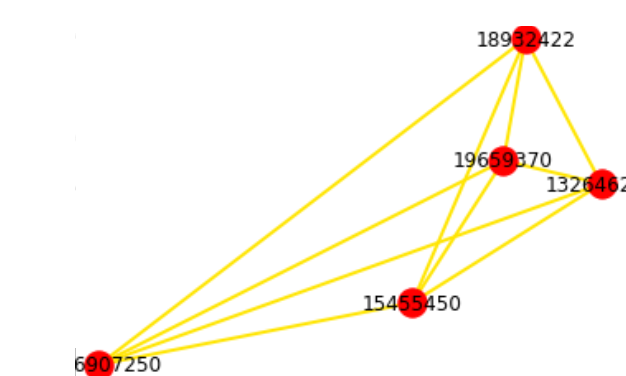
\includegraphics[height=0.35\linewidth]{cricca_kevin}
	\label{fig:criccakevin}
\end{figure}

Vista la complessità computazionale dell'operazione di \textbf{maxClique}, l'abbiamo applicata su uno dei sottografi più piccoli del grafo principale. Notiamo nella cricca massima la presenza di un nodo utente al di fuori dei nodi principali (15455450).
\pagebreak
\section{Smallworldness}
Considerando il sottografo non direzionato il valore dei parametri:
	\begin{itemize}
	\item Omega: 0.00307
	\item Sigma: 0.9808
\end{itemize}
Il valore di omega vicino allo 0, indica che il grafo ha le caratteristiche di una rete piccolo mondo.
Dato confermato anche dal valore di Sigma vicino ad 1.
I parametri sono stati calcolati con:\newline
- niter = 15, indica il numero approssimativo di ridirezioni per arco, per calcolare il grafico casuale equivalente\newline
- nrand = 4, indica il numero di grafici casuali generati per calcolare il coefficiente di clustering medio e la lunghezza del percorso medio più breve.\newline
Abbiamo optato per valori più bassi rispetto a quelli di default (100,10), questo per ridurre la complessità computazionale del calcolo dei parametri.
\section{Analisi delle correlazioni di Pearson e Kendall}

\begin{figure}[h]
	\centering
	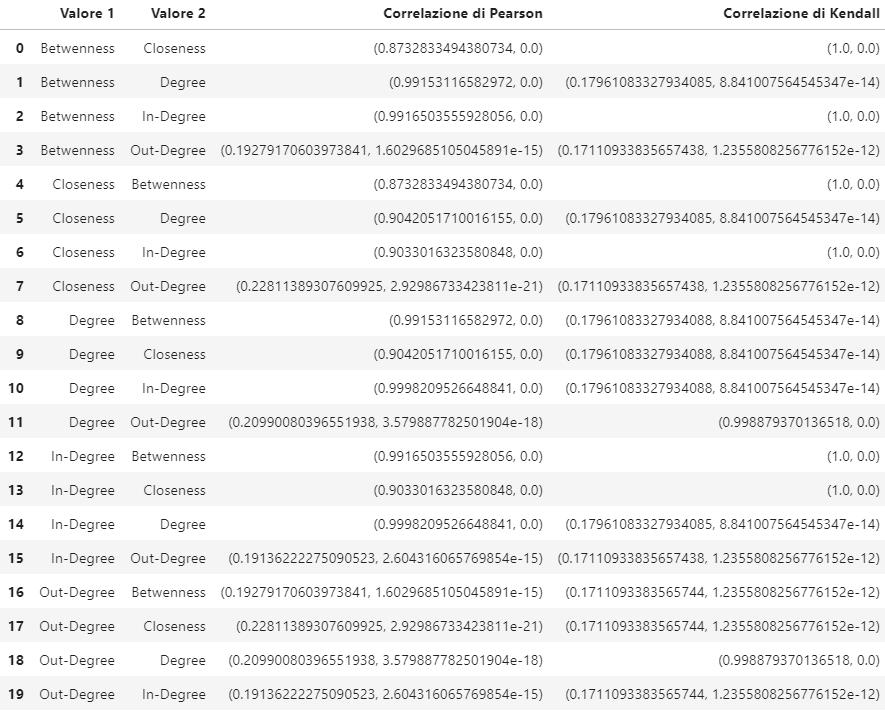
\includegraphics[width=1\linewidth]{tabella}
	\caption[]{Tabella della Correlazione di Pearson e Kendel relativa alle misure di centralità del grafo}
\end{figure}
Nella tabella è indicato nella terza colonna il valore di correlazione di Pearson e nella quarta colonna il valore di correlazione di Kendall.
Nella terza colonna i valore vicini all'1 indicano la presenza di correlazione lineare tra il primo ed il secondo parametro, per esempio la \textbf{Betweenness centrality} e la \textbf{In-degree centrality} sono decisamente correlate, rispetto ad esempio la \textbf{Betweenness centrality} e l'\textbf{Out-degree centrality}



\end{document}